\chapter{Taking Advantage of the Internet}


  % location of 
    % not sure this does anything unless we use pgfSweave
         % keep.source probably disables this
          % use pdf for graphics
  % remove blank lines at beginning and end 
  % keeps formatting from original; allows ? to work


\section{Google Docs and \RStudio}

\section{Sharing in \RStudio}

\section{Other Ways to Make Data Available Online}

\section{Data Mining Activities}
\subsection{What percentage of Earth is Covered with Water?}
We can estimate the proportion of the world covered with water by randomly 
sampling points on the globe and inspecting them using GoogleMaps.

First, let's do a sample size computation.  Suppose we want to 
estimate (at the 95\% confidence level) this proportion with $\pm 5$\%.
There are several ways to estimate the necessary sample size, including
algebraically solving
\[
(1.96) \sqrt{ \hat p (1-\hat p) /n} = 0.05
\]
for $n$ given some estimated value of $p$.  The \verb!uniroot()! function
can solve this sort of thing numerically.  Here we take an approach 
that looks at a table of values of $n$ and $\hat p$ and margin of error.
\begin{Schunk}
\begin{Sinput}
> n <- seq(50,500, by=50)
> p.hat <- seq(.5, .9, by=0.10)
> margin_of_error <- function(n, p, conf.level=.95) { 
+ 	-qnorm( (1-conf.level)/2) * sqrt( p * (1-p) / n ) 
+ }
> outer(n, p.hat, margin_of_error) -> tbl
> colnames(tbl) <- p.hat
> rownames(tbl) <- n
> tbl
\end{Sinput}
\begin{Soutput}
           0.5        0.6        0.7        0.8        0.9
50  0.13859038 0.13579029 0.12702018 0.11087231 0.08315423
100 0.09799820 0.09601823 0.08981683 0.07839856 0.05879892
150 0.08001519 0.07839856 0.07333514 0.06401216 0.04800912
200 0.06929519 0.06789514 0.06351009 0.05543615 0.04157711
250 0.06197950 0.06072726 0.05680515 0.04958360 0.03718770
300 0.05657929 0.05543615 0.05185577 0.04526343 0.03394757
350 0.05238224 0.05132390 0.04800912 0.04190579 0.03142934
400 0.04899910 0.04800912 0.04490842 0.03919928 0.02939946
450 0.04619679 0.04526343 0.04234006 0.03695744 0.02771808
500 0.04382613 0.04294066 0.04016731 0.03506090 0.02629568
\end{Soutput}
\end{Schunk}
From this it appears that a sample size of approximately 300--400 will get
us the accuracy we desire.  A class of students can easily generate
this much data in a matter of minutes if each student inspects 10--20 maps.
The example below assumes a sample size of 10 locations per student.
This can be adjusted depending on the number of students and the desiered
margin of error.

\begin{enumerate}
\item Generate 10 random locations.

\begin{Schunk}
\begin{Sinput}
> positions <- rgeo(10); positions
\end{Sinput}
\begin{Soutput}
         lat        lon
1  -35.86447  -73.08316
2  -45.84062 -179.52211
3   53.96125   13.78336
4  -59.79423  161.11034
5   23.31866   23.36082
6  -51.59494  -99.90623
7   67.40824  159.25404
8   45.08550  -72.15787
9   10.25286   56.03133
10 -28.51074  -31.39516
\end{Soutput}
\end{Schunk}

\item
Open a GoogleMap centered at each position.

\begin{Schunk}
\begin{Sinput}
> googleMap(pos=positions, mark=TRUE)
\end{Sinput}
\end{Schunk}
You may need to turn off pop-up block for this to work smoothly.

\item
For each map, record whether the center is located in water or on land.  \verb!mark=TRUE!
is used to place a marker at the center of the map which is helpful for locations that are close to 
the coast.  
\begin{center}
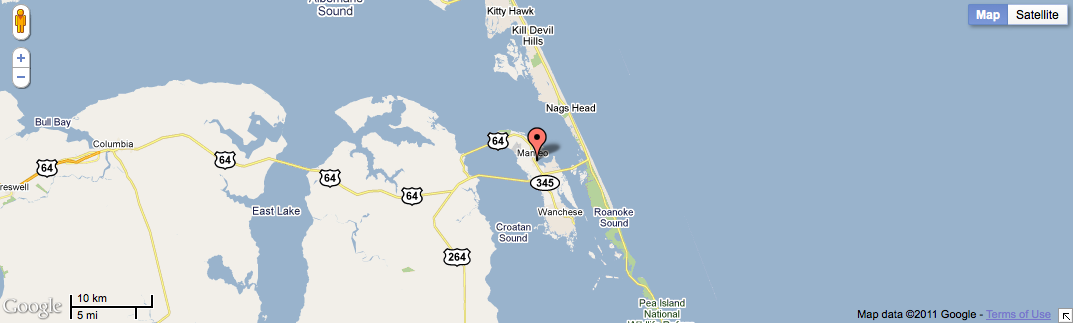
\includegraphics[width=.8\textwidth]{images/google-water1}
\end{center}
You can zoom in or out to get a better look.
\begin{center}
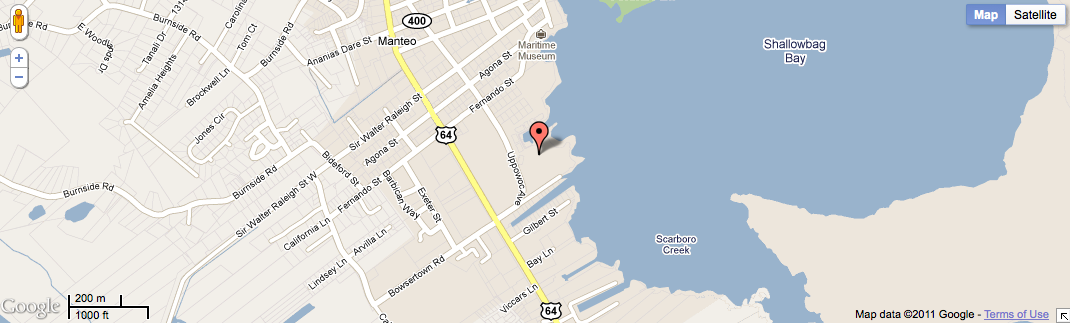
\includegraphics[width=.8\textwidth]{images/google-water2}
\end{center}


\item
Record your data in a GoogleForm at 

\begin{center}
\url{https://spreadsheets.google.com/viewform?formkey=dGREcUR6YjRLSWFTWVpNNXA5ZUZ1TXc6MQ}

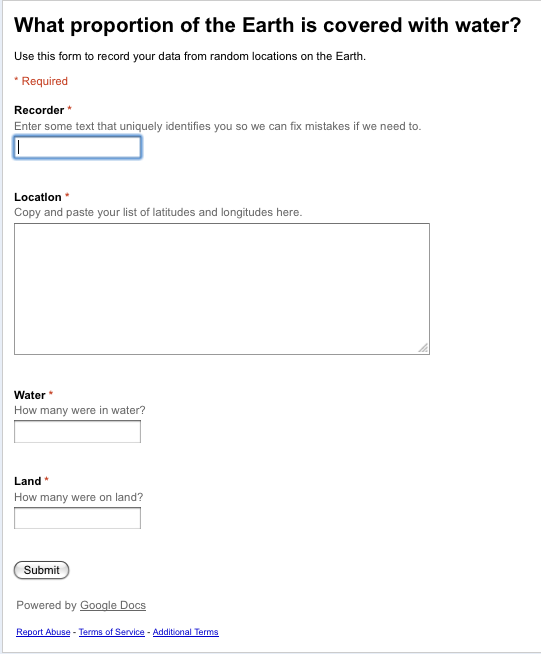
\includegraphics[width=.4\textwidth]{images/googleForm-water}
\end{center}

For the latitude and longitude information, simply copy and paste the output of 
\begin{Schunk}
\begin{Sinput}
> positions
\end{Sinput}
\end{Schunk}
\item
After importing the data from Google, it is simple to sum the counts across the class.


\begin{Schunk}
\begin{Sinput}
> sum(Water$Water)
\end{Sinput}
\begin{Soutput}
[1] 215
\end{Soutput}
\begin{Sinput}
> sum(Water$Land)
\end{Sinput}
\begin{Soutput}
[1] 85
\end{Soutput}
\end{Schunk}

Then use your favorite method of analysis, perhaps \verb!binom.test()!.

\begin{Schunk}
\begin{Sinput}
> interval(binom.test(215,300))
\end{Sinput}
\begin{Soutput}
Method: Exact binomial test

probability of success 
             0.7166667 

95% confidence interval: 
0.662036 0.7669599
\end{Soutput}
\end{Schunk}
\end{enumerate}


\subsection{Roadless America}

The \verb!rgeo()! can also sample within a latitude longitude ``rectangle".
This allows us to sample subsets of the globe.  In this activity we will estimate 
the proportion of the continental United States that is within 1 mile of a road.

\begin{enumerate}
\item
Generate a random sample of locations in a box containing the continental United States.
Some of these points may be in Canada, Mexico, an ocean or a major lake.  These 
will be discarded from our sample before making our estimate.
\begin{Schunk}
\begin{Sinput}
> positions <- rgeo(10, lonlim=c(-125,-65), latlim=c(25,50)); positions
\end{Sinput}
\begin{Soutput}
        lat        lon
1  40.45280  -89.33939
2  33.71560  -72.13336
3  43.99032  -94.07041
4  31.38016  -70.94796
5  35.95121 -104.26389
6  39.13885  -65.56925
7  44.41212  -78.94507
8  42.15868  -93.90161
9  29.79189  -97.81417
10 45.99380  -82.01440
\end{Soutput}
\end{Schunk}

\item
Open a GoogleMap centered at each position.  This time we'll zoom in a bit and add 
a circle of radius 1 to our map.

\begin{Schunk}
\begin{Sinput}
> googleMap(pos=positions, mark=TRUE, zoom=12, radius=1)
\end{Sinput}
\end{Schunk}


\begin{center}
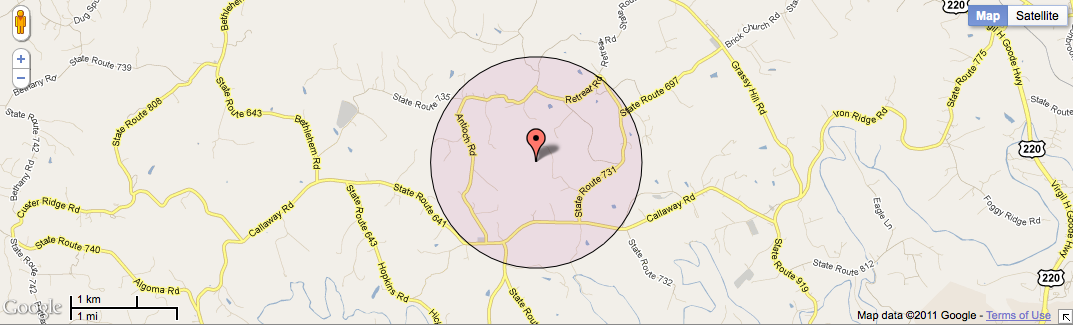
\includegraphics[width=.8\textwidth]{images/google-roadless}
\end{center}
You may need to turn off pop-up block for this to work smoothly.
\item
For each map, record whether the center is close (to a road), far (from a road), water, or foreign.
You may need to zoom in or out a bit to figure this out.

\end{enumerate}

\subsection{Variations on the Google Maps theme}

There are many other quantities one could estimate using these tools.  For example:
\begin{enumerate}
\item
What proportion of you home state is within $m$ miles of a lake?  (The choice of $m$ may depend upon
your state of interest.)
\item
Use two proportion procedures  or chi-squared tests to compare states or continents.  
Do all continents have roughly the same proportion of land withing $m$ miles of water (for some $m$)?
Are Utah and Arizona equally roadless?

\item
In more advanced classes: What is the average distance to the nearest lake (in some region)?
By using concentric circles, one could estimate this from discretized data indicating, for example,
whether the nearest lake is within 1/2 mile, between 1/2 mile and 1 mile, between 1 mile and 2 miles,
between 2 miles, and 4 miles, between 4 miles and 10 miles, or more than 10 miles away.  It may be 
interesting to discuss what sort of model should be used for distances from random locations to lakes.
(It probably isn't normally distributed.)
\authNote{Is this example too complicated?}%
\end{enumerate}

\subsection{Zillow}
Nick 

